\section{条件分布的定义}
\label{sec:cdis-definition}

第~\ref{chap:random-vectors}章用两种具体表示计算条件分布。有概率表时，取出$Y=y$对应的一列（或一行），除以它的和；有联合密度时，取出$Y=y$处的切片，除以边缘密度$f_Y(y)$。两种做法都对每个观测值$y$给出$X$的一个分布。没有概率表也没有密度时，这件事怎样做？本节先把单个事件的条件概率写成条件期望，再引入一个对象，同时记录所有目标事件的条件概率，最后要求它与原来的联合规律相容。

全章的设定如下。$(\Omega,\mathcal{F},\mathbb{P})$是概率空间，$X$是取值于可测空间$(\mathcal{X},\mathcal{F}_{\mathcal{X}})$的随机对象，$Y$是取值于$(\mathcal{Y},\mathcal{F}_{\mathcal{Y}})$的随机对象，$\mathcal{G}\subseteq\mathcal{F}$是一个子$\sigma$代数，代表已知的信息。$X$是我们想了解的目标，$Y$或$\mathcal{G}$是已经掌握的条件。

\subsection{给定信息的条件概率}
\label{sec:cdis-conditional-probability}

事件的概率是指示函数的期望：
\[
 \mathbb{P}(X\in A)=\mathbb{E}\bigl[\mathbf{1}_{\{X\in A\}}\bigr].
\]
第~\ref{chap:conditional-expectation}章对任意可积随机变量定义了给定$\mathcal{G}$的条件期望，指示函数有界，当然可积。于是条件概率可以直接借用条件期望来定义。

\begin{definition}[给定信息的条件概率]
\label{def:cdis-conditional-probability}
对$A\in\mathcal{F}_{\mathcal{X}}$，称
\begin{equation}
 \mathbb{P}(X\in A\mid\mathcal{G})=\mathbb{E}\bigl[\mathbf{1}_{\{X\in A\}}\bigm|\mathcal{G}\bigr]
 \label{eq:cdis-conditional-probability}
\end{equation}
为给定$\mathcal{G}$时事件$\{X\in A\}$的条件概率。给定随机对象$Y$时取$\mathcal{G}=\sigma(Y)$，记作$\mathbb{P}(X\in A\mid Y)$。
\end{definition}

条件概率是一个随机变量，不是一个数。它的取值随样本点$\omega$改变，但只能通过$\mathcal{G}$所能区分的信息改变；它在已知的每个事件$G\in\mathcal{G}$上保留原来的累计概率：
\[
 \mathbb{E}\bigl[\mathbf{1}_{G}\,\mathbb{P}(X\in A\mid\mathcal{G})\bigr]=\mathbb{P}(\{X\in A\}\cap G).
\]
按第~\ref{chap:conditional-expectation}章的结论，它只在零概率集之外确定；满足定义的任何一个随机变量都称为它的一个版本。

\paragraph{有限分组中的条件概率}
先看两台传感器。联合概率表关于对角线对称，两台读数的边缘都是$(0.3,0.4,0.3)$。取目标事件$\{X=2\}$、条件$Y$。$\sigma(Y)$把样本空间分成三组$\{Y=0\},\{Y=1\},\{Y=2\}$，每组概率为正，组内的条件概率就是组内的比例：
\[
 \frac{0}{0.3}=0,\qquad \frac{0.10}{0.4}=\frac14,\qquad \frac{0.20}{0.3}=\frac23.
\]
所以$\mathbb{P}(X=2\mid Y)$是一个随机变量，它在$Y=0,1,2$时分别取$0,\tfrac14,\tfrac23$，相应的概率是$0.3,0.4,0.3$。

再按组的概率加权平均，得到
\[
 \mathbb{E}\bigl[\mathbb{P}(X=2\mid Y)\bigr]=0.3\cdot0+0.4\cdot\tfrac14+0.3\cdot\tfrac23=0.3=\mathbb{P}(X=2).
\]
这就是在已知事件$G=\Omega$上保留累计概率。三组的值各不相同，说明知道第二台的读数会改变我们对“第一台读偏高”的判断。

\paragraph{给定观测的函数表示}
给定$Y$时，第~\ref{chap:conditional-expectation}章说明$\sigma(Y)$可测的随机变量都能写成$Y$的可测函数。对每个$A$，存在可测函数$h_A:\mathcal{Y}\to[0,1]$，使
\begin{equation}
 \mathbb{P}(X\in A\mid Y)=h_A(Y)\quad\text{几乎必然}.
 \label{eq:cdis-function-representation}
\end{equation}
代入观测值，记$\mathbb{P}(X\in A\mid Y=y)=h_A(y)$。这个函数只在$Y$的分布$P_Y$下几乎处处确定：在一个$P_Y$零测集上改动$h_A$，式~\eqref{eq:cdis-function-representation}仍然成立。

三角形模型中，第~\ref{chap:random-vectors}章已经求出给定$Y=y$（$0\leq y<1$）时$X$在$[y,1]$上均匀分布。取$A=[\tfrac34,1]$，区间$[y,1]$中落在$A$内的长度占比就是$h_A(y)$：
\[
 h_A(y)=\begin{cases}
 \dfrac{1}{4(1-y)}, & 0\leq y\leq\tfrac34,\\
 1, & \tfrac34<y<1.
 \end{cases}
\]
它随$y$增大而增大：较小的读数越大，较大的读数越有可能落在$[\tfrac34,1]$中；$y>\tfrac34$时，$X\geq Y$已经保证$X\in A$。

图~\ref{fig:cdis-event-function}把这个随机变量画在样本空间上。(a)中三角形内每一点$(x,y)$的颜色是$h_A(y)$，颜色只随纵坐标改变，同一条水平线上颜色相同：条件概率只用到$Y$所携带的信息。(b)是函数$h_A$本身。

\begin{BookInlineFigure}
  \centering
  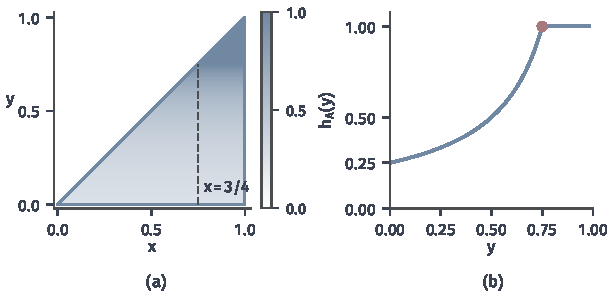
\includegraphics[width=104mm]{figures/07-probability/02-measure-theoretic-probability/matplotlib/cdis-event-function/figure.pdf}
  \caption{三角形模型中的条件概率$\mathbb{P}(X\in A\mid Y)$，$A=[\tfrac34,1]$。(a)三角形内一点$(x,y)$的颜色深浅表示$h_A(y)$，由白到蓝逐渐增大；颜色只随$y$变化，虚线$x=\tfrac34$左侧的点不在事件$\{X\in A\}$中，却与右侧同一水平线上的点取相同的值。(b)蓝线是$h_A(y)$，红点标出$y=\tfrac34$，此后$h_A=1$。}
  \label{fig:cdis-event-function}
\end{BookInlineFigure}

\paragraph{逐事件的概率规则}
条件概率是否像概率一样运算？非负、总量为一可以从条件期望的保序与线性直接得到；可数可加涉及无穷和，需要一个与积分的单调收敛定理对应的结论。

\begin{lemma}[条件单调收敛]
\label{lem:cdis-conditional-monotone}
设$0\leq Z_1\leq Z_2\leq\cdots$，$Z_n\to Z$，且$\mathbb{E}[Z]<\infty$。则$\mathbb{E}[Z_n\mid\mathcal{G}]$几乎必然递增地收敛到$\mathbb{E}[Z\mid\mathcal{G}]$。
\end{lemma}

\begin{proof}
由条件期望的保序性，对每个$n$，几乎必然有
\[
 0\leq\mathbb{E}[Z_n\mid\mathcal{G}]\leq\mathbb{E}[Z_{n+1}\mid\mathcal{G}]\leq\mathbb{E}[Z\mid\mathcal{G}].
\]
这是可数多个关系，例外集的并$N$仍是零概率集，并且$N\in\mathcal{G}$，因为它由$\mathcal{G}$可测的函数之间的比较定义。

在$N$之外令$W=\lim_n\mathbb{E}[Z_n\mid\mathcal{G}]$，在$N$上令$W=0$。$W$是$\mathcal{G}$可测函数的极限，因而$\mathcal{G}$可测，并且$0\leq W\leq\mathbb{E}[Z\mid\mathcal{G}]$几乎必然，所以可积。任取$G\in\mathcal{G}$，对递增的非负列两次使用单调收敛定理，得到
\[
 \mathbb{E}[\mathbf{1}_{G}W]=\lim_{n\to\infty}\mathbb{E}\bigl[\mathbf{1}_{G}\,\mathbb{E}[Z_n\mid\mathcal{G}]\bigr]=\lim_{n\to\infty}\mathbb{E}[\mathbf{1}_{G}Z_n]=\mathbb{E}[\mathbf{1}_{G}Z].
\]
中间的等号是条件期望在$G$上的积分恒等式。$W$满足条件期望的定义，由唯一性，$W=\mathbb{E}[Z\mid\mathcal{G}]$几乎必然。
\end{proof}

\begin{lemma}[逐事件的条件概率规则]
\label{lem:cdis-eventwise-rules}
对任意$A\in\mathcal{F}_{\mathcal{X}}$，几乎必然有$0\leq\mathbb{P}(X\in A\mid\mathcal{G})\leq1$，且$\mathbb{P}(X\in\mathcal{X}\mid\mathcal{G})=1$。对任意一列两两不交的$A_1,A_2,\ldots\in\mathcal{F}_{\mathcal{X}}$，几乎必然有
\begin{equation}
 \mathbb{P}\Bigl(X\in\bigcup_{n}A_n\Bigm|\mathcal{G}\Bigr)=\sum_{n}\mathbb{P}(X\in A_n\mid\mathcal{G}).
 \label{eq:cdis-eventwise-additivity}
\end{equation}
\end{lemma}

\begin{proof}
$0\leq\mathbf{1}_{\{X\in A\}}\leq1$，由保序性得到第一条；$\mathbf{1}_{\{X\in\mathcal{X}\}}=1$是常数，常数的条件期望是它自己。对不交的$A_n$，部分和$\sum_{k\leq n}\mathbf{1}_{\{X\in A_k\}}$递增地收敛到$\mathbf{1}_{\{X\in\cup_kA_k\}}$。由线性，部分和的条件期望是各项条件期望之和；再由引理~\ref{lem:cdis-conditional-monotone}取极限，得到式~\eqref{eq:cdis-eventwise-additivity}。
\end{proof}

引理中的“几乎必然”有一个容易忽略的限定：例外集依赖于所取的事件或事件列。对每个固定的$A$，总可以在一个零概率集之外谈论$\mathbb{P}(X\in A\mid Y=y)$；可是事件有不可数多个，不同事件的例外集合并起来可能不再是零概率集。于是出现一个问题：能否为每个$A$选定一个版本$h_A$，使对每个（或几乎每个）观测值$y$，映射$A\mapsto h_A(y)$都是$\mathcal{X}$上的一个概率分布？下面先给这样的对象一个名称。

\subsection{概率核}
\label{sec:cdis-kernel}

概率表给出了最简单的模型。传感器表按列$y$取出、除以列和，得到三个条件分布；把它们排成矩阵，每一行对应一个观测值，每行非负且和为$1$。这样的矩阵同时记录了所有目标事件的条件概率：给定$Y=y$时$X\in A$的概率，就是第$y$行在$A$中的元素之和。

\begin{BookInlineFigure}
  \centering
  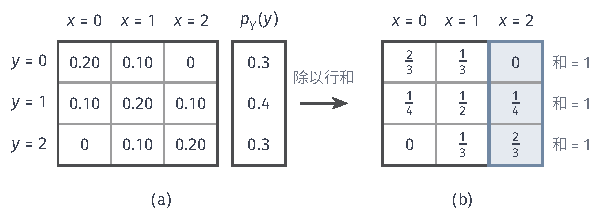
\includegraphics[width=102mm]{figures/07-probability/02-measure-theoretic-probability/tikz/cdis-table-kernel/figure.pdf}
  \caption{由传感器的联合概率表得到概率核。(a)联合概率表，行是第二台读数$y$，列是第一台读数$x$，右侧是行和$p_Y(y)$。(b)每行除以行和得到的矩阵$K(y,\{x\})$，每行是一个概率分布；浅蓝格子组成事件$\{X=2\}$所在的列，它的各行元素就是$\mathbb{P}(X=2\mid Y=y)$。}
  \label{fig:cdis-table-kernel}
\end{BookInlineFigure}

图~\ref{fig:cdis-table-kernel}画出这一步。对$A=\{2\}$，(b)中浅蓝一列给出$0,\tfrac14,\tfrac23$，正是上一小节逐个算出的条件概率；对其他事件，只要换成对应的列求和。一般情形要求的就是这样一个按观测值排列的分布族。

\begin{definition}[概率核]
\label{def:cdis-kernel}
设映射$K$对每个$y\in\mathcal{Y}$与$A\in\mathcal{F}_{\mathcal{X}}$给出一个数$K(y,A)\in[0,1]$。若
\begin{enumerate}
 \item 对每个$y\in\mathcal{Y}$，$A\mapsto K(y,A)$是$(\mathcal{X},\mathcal{F}_{\mathcal{X}})$上的概率测度；
 \item 对每个$A\in\mathcal{F}_{\mathcal{X}}$，$y\mapsto K(y,A)$是$\mathcal{F}_{\mathcal{Y}}$可测函数，
\end{enumerate}
则称$K$为从$(\mathcal{Y},\mathcal{F}_{\mathcal{Y}})$到$(\mathcal{X},\mathcal{F}_{\mathcal{X}})$的\term{概率核}（probability kernel），也称转移核。按测度的写法，$K(y,A)$也写成
\begin{equation}
 K(y,A)=\int_{A}K(y,\mathrm{d}x).
 \label{eq:cdis-kernel-notation}
\end{equation}
\end{definition}

两项要求各有用处。第一项是概率表“每行归一”的推广：固定观测值，得到一个完整的分布，事件之间的可加性对这个$y$处处成立，不再附带依赖事件的例外集。第二项保证固定事件$A$后，$K(\cdot,A)$是$\mathcal{Y}$上的可测函数，因而可以按$Y$的分布积分，例如计算$\int_{B}K(y,A)\,P_Y(\mathrm{d}y)$。$\mathcal{Y}$有限且每个子集都可测时，第二项自动成立，所以在概率表中只看得到第一项。

第二项并非多余。设$S\subseteq[0,1]$不是Borel集，令$y\in S$时$K(y,\cdot)$是$\{1\}$上的单点分布，其余$y$时是$\{0\}$上的单点分布。每个$K(y,\cdot)$都是概率测度，但$y\mapsto K(y,\{1\})=\mathbf{1}_{S}(y)$不可测，积分$\int K(y,\{1\})\,P_Y(\mathrm{d}y)$没有意义。这样的$K$无法用来“按观测加权”，也就谈不上与联合规律相容。

\paragraph{三角形模型的核}
三角形模型中，对$0\leq y<1$令$K(y,\cdot)$为$[y,1]$上的均匀分布，记$\lambda$为长度，则
\[
 K(y,A)=\frac{\lambda(A\cap[y,1])}{1-y},\qquad 0\leq y<1,
\]
在$y=1$等其余点令$K(y,\cdot)$为$\{1\}$上的单点分布。固定$y$，这是一个概率测度。固定$A$，函数$y\mapsto\lambda(A\cap[y,1])$连续，因而$K(\cdot,A)$在$[0,1)$上可测，补上可测的余下部分后整体可测。

图~\ref{fig:cdis-kernel-views}从两个方向看同一个核。(a)固定观测值，曲线是分布函数$t\mapsto K(y,[0,t])$：每个$y$对应一个完整的分布。(b)固定事件，曲线是观测值的函数$y\mapsto K(y,A)$：每个事件对应一个可测函数。概率核的定义就是要求这两个方向同时成立。

\begin{BookInlineFigure}
  \centering
  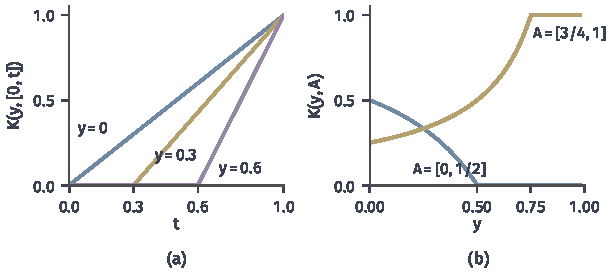
\includegraphics[width=104mm]{figures/07-probability/02-measure-theoretic-probability/matplotlib/cdis-kernel-views/figure.pdf}
  \caption{三角形模型的概率核$K(y,\cdot)=\operatorname{Unif}(y,1)$的两种读法。(a)固定$y=0,0.3,0.6$（蓝、黄、紫），横轴为$t$，曲线为$K(y,[0,t])$，每条都是一个分布函数。(b)固定事件$A=[0,\tfrac12]$（蓝）与$A=[\tfrac34,1]$（黄），曲线为$y\mapsto K(y,A)$。}
  \label{fig:cdis-kernel-views}
\end{BookInlineFigure}

\paragraph{核对函数与对测度的作用}
概率表的核是行和为一的非负矩阵，它可以从右边乘列向量，也可以从左边乘行向量。一般的核同样有这两种作用。对有界可测函数$g$，令$(Kg)(y)=\int g(x)\,K(y,\mathrm{d}x)$，这是“观测为$y$时$g$的平均”；对$\mathcal{Y}$上的概率测度$\mu$，令$(\mu K)(A)=\int K(y,A)\,\mu(\mathrm{d}y)$，这是“先按$\mu$抽观测值、再按核抽目标”时目标的分布。第~\ref{sec:cdis-integration}节与第~\ref{sec:cdis-joint}节分别研究这两种作用；概率表中它们就是矩阵乘列向量与行向量乘矩阵。

\subsection{正则条件分布}
\label{sec:cdis-regular}

概率核本身只是一族按观测值排列的分布，与$X$、$Y$的联合规律还没有关系。任意一个核都满足定义~\ref{def:cdis-kernel}，例如对所有$y$都取同一个分布。要让它成为“给定$Y$时$X$的分布”，必须要求它在每个事件上给出的值就是条件概率。

\begin{definition}[正则条件分布]
\label{def:cdis-regular}
从$\mathcal{Y}$到$\mathcal{X}$的概率核$K$若对每个$A\in\mathcal{F}_{\mathcal{X}}$满足
\begin{equation}
 K(Y,A)=\mathbb{P}(X\in A\mid Y)\quad\text{几乎必然},
 \label{eq:cdis-regular}
\end{equation}
则称$K$为给定$Y$时$X$的\term{正则条件分布}（regular conditional distribution），也记作$P_{X\mid Y}(A\mid y)=K(y,A)$。
\end{definition}

式~\eqref{eq:cdis-regular}中的例外集仍然可以随$A$改变，这一点与逐事件的条件概率相同。差别在于，核对每个$y$都是概率测度：正则条件分布是从条件概率的众多版本中挑出的一组，使得在每个观测值处都拼成一个分布。“正则”指的就是这种可以拼合的性质。给定一般的信息$\mathcal{G}$时，把$\mathcal{Y}$换成$(\Omega,\mathcal{G})$、$Y$换成恒等映射，同样可以定义给定$\mathcal{G}$的正则条件分布，本章主要讨论给定随机对象$Y$的情形。

验证一个核是否满足式~\eqref{eq:cdis-regular}，按条件期望的定义需要检查$\sigma(Y)$中的每个事件。$\sigma(Y)$的事件都形如$\{Y\in B\}$，把这一检查写成$\mathcal{Y}$上的积分，得到一个便于计算的判别。

\begin{lemma}[正则条件分布的积分判别]
\label{lem:cdis-regular-criterion}
概率核$K$是给定$Y$时$X$的正则条件分布，当且仅当对一切$A\in\mathcal{F}_{\mathcal{X}}$、$B\in\mathcal{F}_{\mathcal{Y}}$，
\begin{equation}
 \mathbb{P}(X\in A,\ Y\in B)=\int_{B}K(y,A)\,P_Y(\mathrm{d}y).
 \label{eq:cdis-regular-criterion}
\end{equation}
\end{lemma}

\begin{proof}
固定$A$。$K(\cdot,A)$可测且取值于$[0,1]$，所以$K(Y,A)$是$\sigma(Y)$可测的有界随机变量。按条件期望的定义，式~\eqref{eq:cdis-regular}成立当且仅当对每个$\{Y\in B\}\in\sigma(Y)$，
\[
 \mathbb{E}\bigl[\mathbf{1}_{\{Y\in B\}}K(Y,A)\bigr]=\mathbb{E}\bigl[\mathbf{1}_{\{Y\in B\}}\mathbf{1}_{\{X\in A\}}\bigr].
\]
右边是$\mathbb{P}(X\in A,\ Y\in B)$。左边的被积函数是$Y$的函数$\mathbf{1}_{B}(y)K(y,A)$，由分布的积分公式（第~\ref{chap:probability-spaces}章），它等于$\int_{B}K(y,A)\,P_Y(\mathrm{d}y)$。两边相等就是式~\eqref{eq:cdis-regular-criterion}。
\end{proof}

式~\eqref{eq:cdis-regular-criterion}说的是：按观测的分布把各个$y$处的条件概率加权累计，必须回到联合概率。这正是“条件化是缩小样本范围再重新归一”的反向检验：把各组重新归一的结果乘回组的质量，应当恢复原来的质量分配。

\paragraph{与概率表和条件密度相容}
有概率表时，取$K(y,\{x\})=p_{X,Y}(x,y)/p_Y(y)$（$p_Y(y)>0$），$p_Y(y)=0$的$y$上任取一个分布。代入式~\eqref{eq:cdis-regular-criterion}的右边，零概率的$y$不贡献，于是
\[
 \sum_{y\in B}p_Y(y)\sum_{x\in A}\frac{p_{X,Y}(x,y)}{p_Y(y)}=\sum_{y\in B}\sum_{x\in A}p_{X,Y}(x,y)=\mathbb{P}(X\in A,\ Y\in B).
\]
第~\ref{chap:random-vectors}章的条件质量函数确实给出正则条件分布。

三角形模型中，$P_Y$有密度$f_Y(y)=2(1-y)$。代入上一小节的核，对$y<1$，$K(y,A)f_Y(y)=2\lambda(A\cap[y,1])$，所以
\[
 \int_{B}K(y,A)\,f_Y(y)\,\mathrm{d}y=\int_{B}\int_{A}2\cdot\mathbf{1}_{\{x\geq y\}}\,\mathrm{d}x\,\mathrm{d}y=\mathbb{P}(X\in A,\ Y\in B).
\]
最后一步是联合密度在$A\times B$上的积分，交换次序的依据是Tonelli定理。一般的条件密度公式在第~\ref{sec:cdis-zero-probability}小节用同样的方法验证。

\paragraph{没有联合密度的情形}
密度比并不是正则条件分布的必要形式。设$Y\sim\operatorname{Unif}(0,1)$，$X=Y$。$(X,Y)$的全部质量落在对角线上，对角线的面积为零，联合密度不存在。直觉上，知道$Y=y$就知道$X=y$，所以应取$K(y,\cdot)=\delta_y$，即$\{y\}$上的单点分布。核对式~\eqref{eq:cdis-regular-criterion}：
\[
 \int_{B}\delta_y(A)\,P_Y(\mathrm{d}y)=P_Y(A\cap B)=\mathbb{P}(Y\in A,\ Y\in B)=\mathbb{P}(X\in A,\ Y\in B).
\]
式~\eqref{eq:cdis-regular-criterion}成立。核$\delta_y$可测：$y\mapsto\delta_y(A)=\mathbf{1}_{A}(y)$对Borel集$A$是可测函数。这个例子说明，正则条件分布的定义不依赖密度，只依赖联合规律本身。
